\section{إعدادات المؤسسة}
\label{sec:settings-feature-organization}

هذه الصفحة هي بطاقة تعريف مؤسستك في النظام: شعاراتها وألوانها وصور صفحتها الرئيسية وعنوانها وقيمها الافتراضية، إضافة إلى ضوابط الملفات المرفقة. تفتحها عند إعداد المؤسسة أول مرة، ثم كلما تغيرت هويتها أو بياناتها. وتؤثر قيمها في جميع الأعضاء، لذلك لا تظهر بطاقتها في «الإعدادات» إلا لمالك المؤسسة.

\begin{rcnote}[مثال: شركة الأفق]
يرفع مسؤول النظام شعار الشركة عند ①، ويختار لونها عند ②، ثم يكتب النطاق الفرعي \en{hzn} ويحفظ الصفحة، فيظهر الشعار واللون لسارة الخطيب وعمر حداد عند دخولهما.
\end{rcnote}

\begin{figure}[H]
\centering
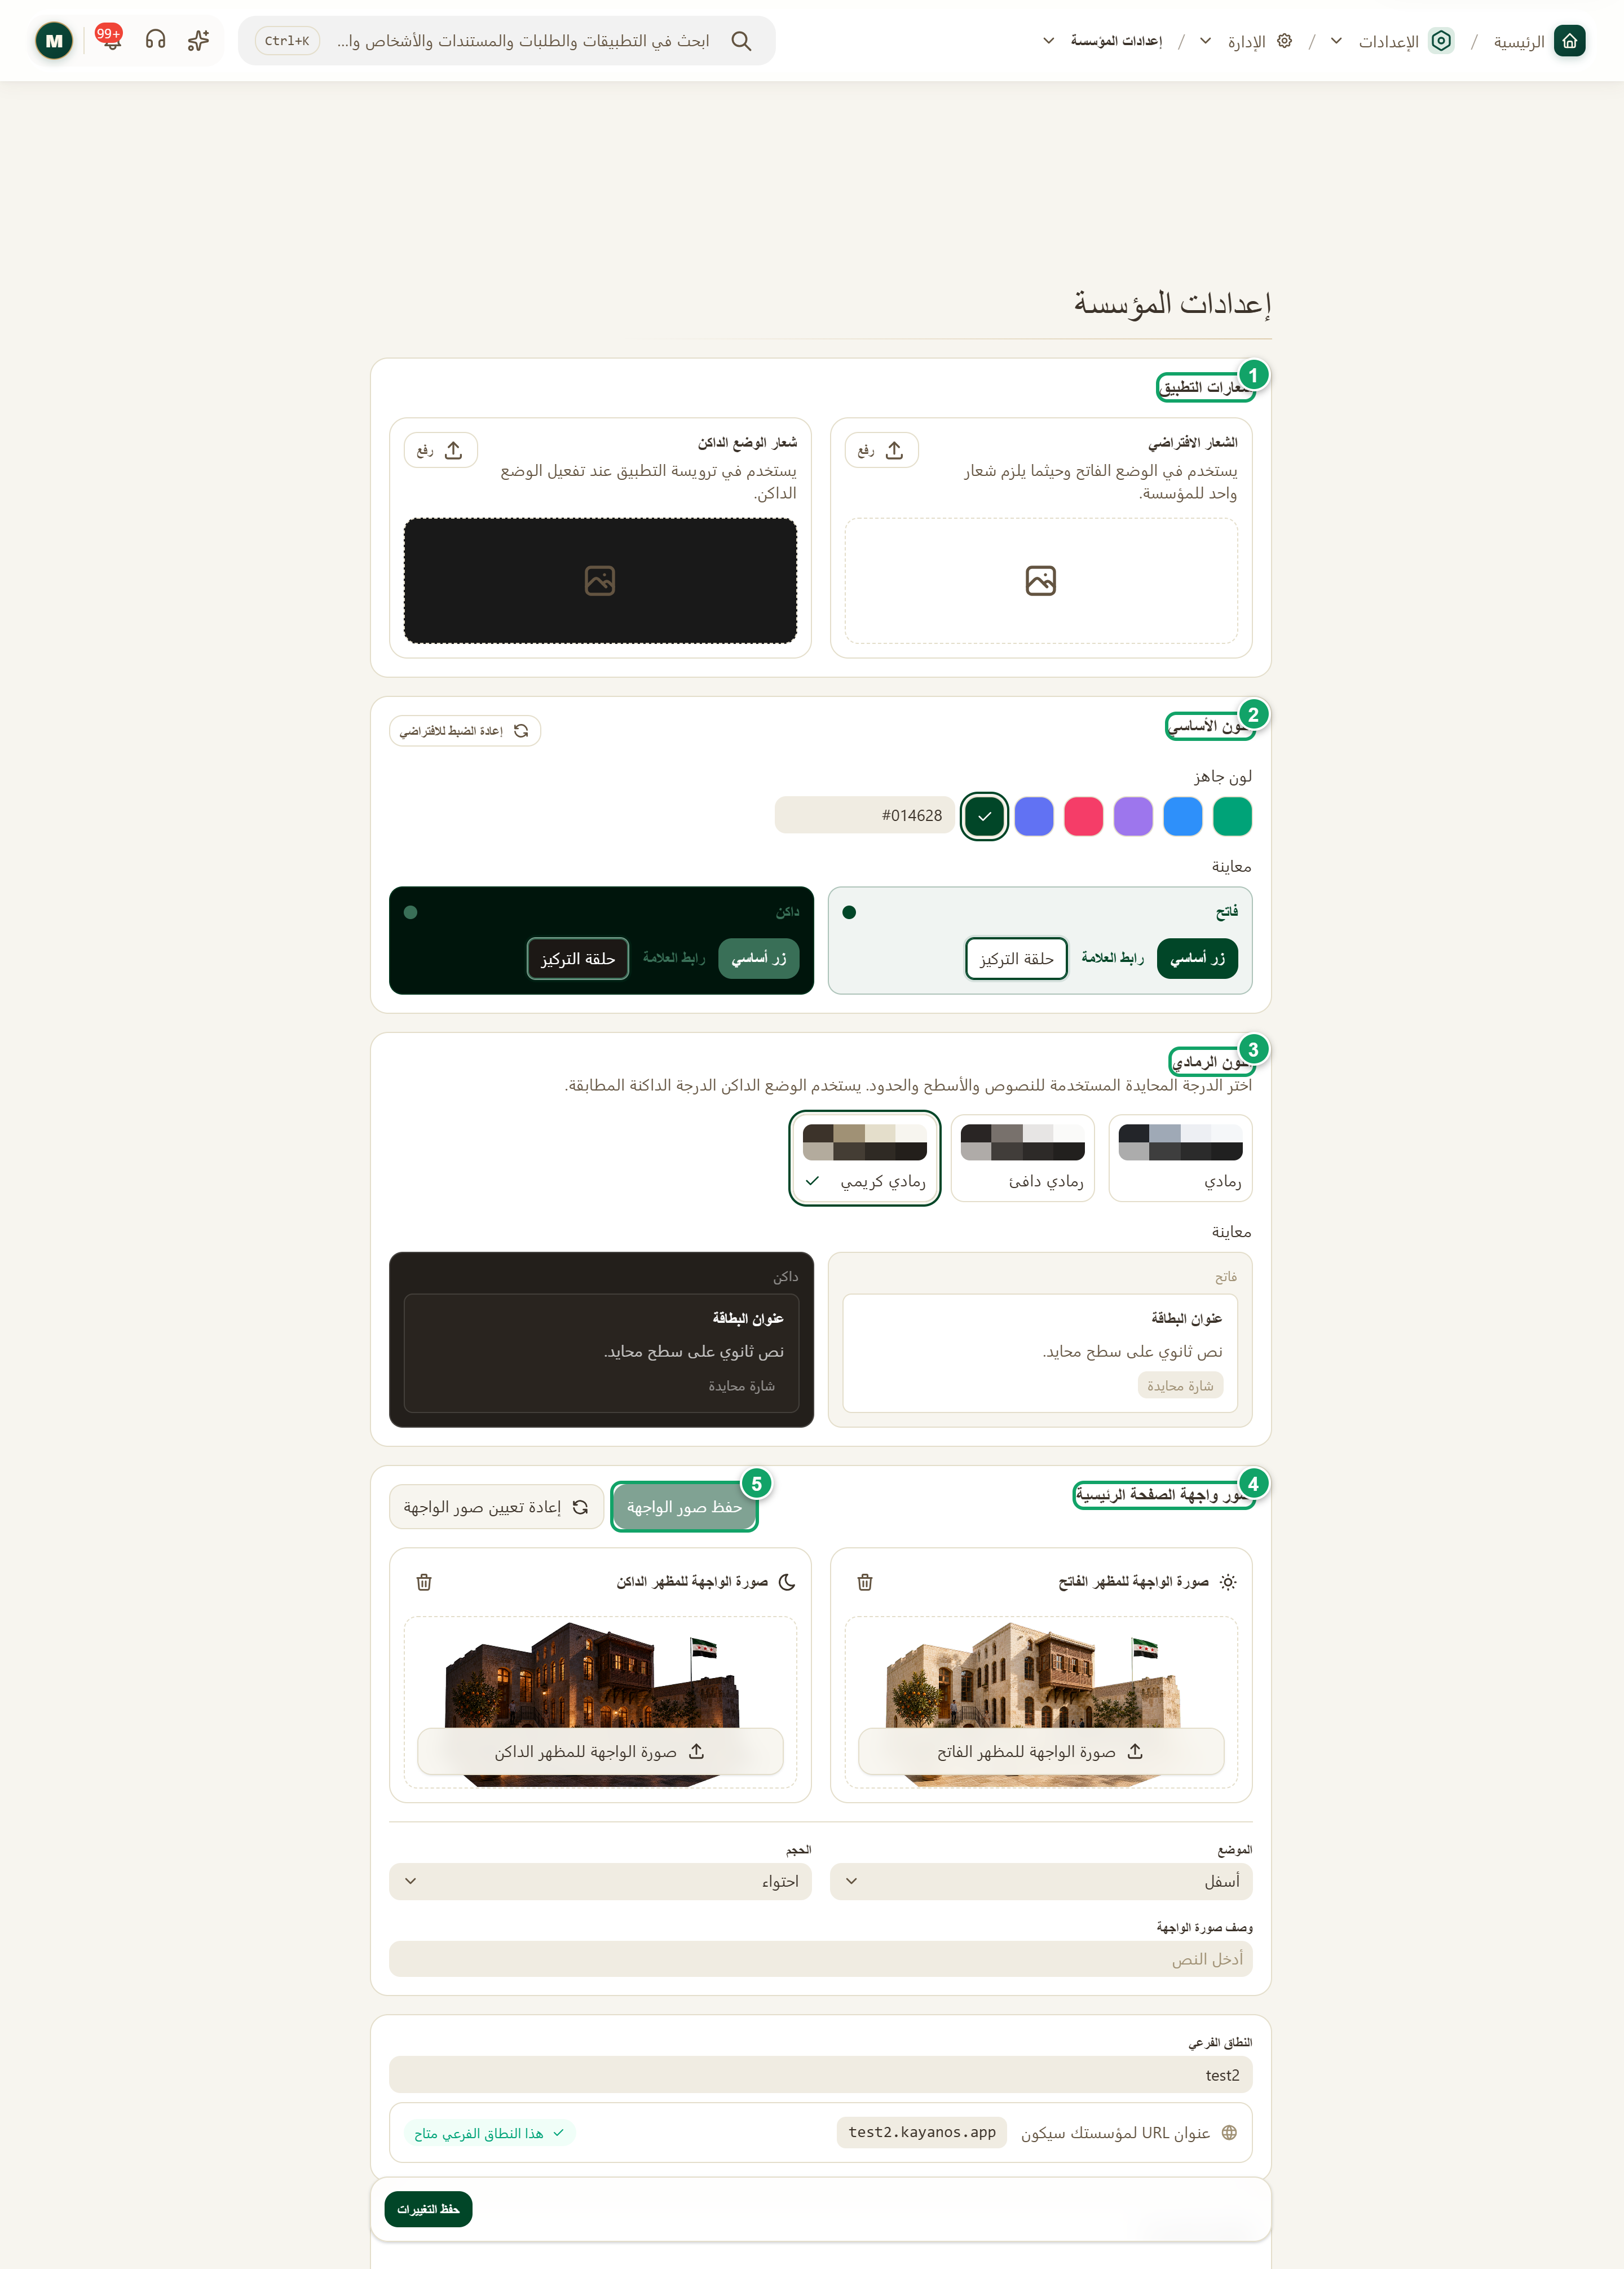
\includegraphics[width=0.95\linewidth,height=0.72\textheight,keepaspectratio]{figures/screens/ch08-organization-ar.png}
\caption{الهوية البصرية للمؤسسة}
\label{fig:settings-organization-screen}
\shotnote{تعرض الصورة القسم البصري من صفحة مؤسسة الاختبار، ولم يُرفع فيها شعار بعد. تعرض بطاقات المعاينة أثر اللون قبل الحفظ، فجرّبه هناك أولاً؛ إذ لا يصل التغيير إلى الأعضاء قبل حفظه. ① «شعارات التطبيق»: شعار للوضع الفاتح وآخر للوضع الداكن. ② «اللون الأساسي»: لون جاهز أو لون مخصص، ويعيد زر «إعادة الضبط للافتراضي» اللون الأصلي. ③ «اللون الرمادي». ④ «صور واجهة الصفحة الرئيسية»: صورتان للمظهرين الفاتح والداكن. ⑤ «حفظ صور الواجهة»: يحفظ الصور وحدها، ويبقى معطلاً حتى تغيّر شيئاً فيها.}
\end{figure}

\begin{figure}[H]
\centering
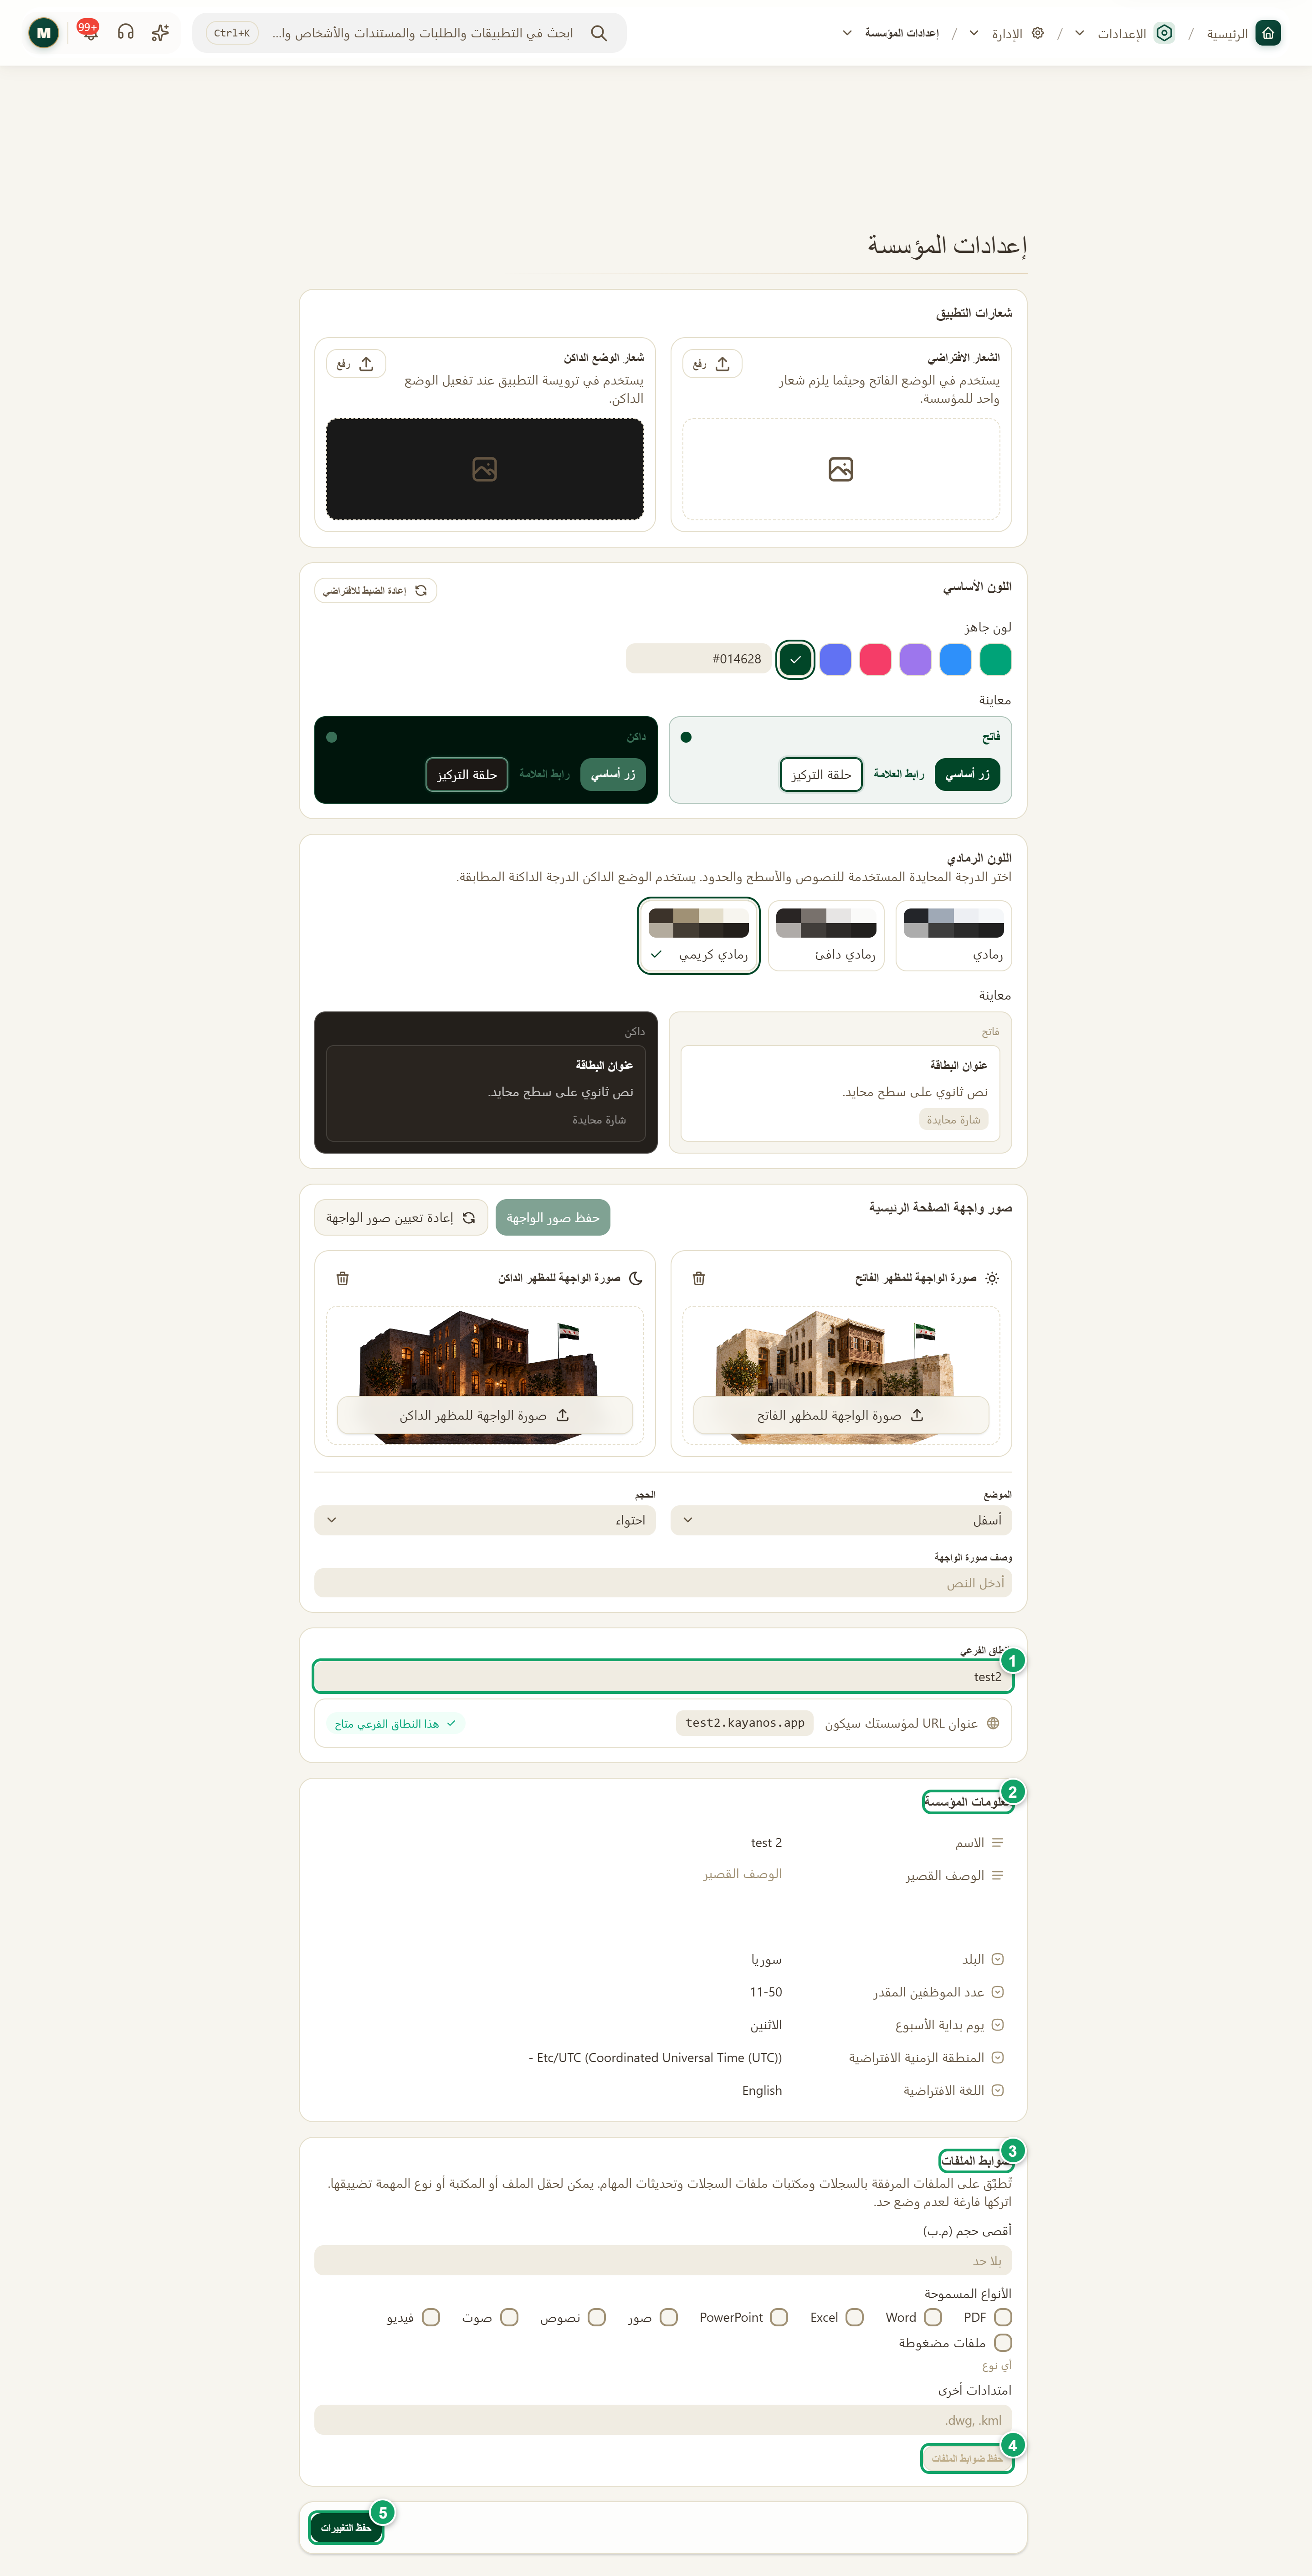
\includegraphics[width=0.95\linewidth,height=0.72\textheight,keepaspectratio]{figures/screens/ch08-organization-info-ar.png}
\caption{العنوان والبيانات وضوابط الملفات}
\label{fig:settings-organization-info-screen}
\shotnote{تعرض الصورة الصفحة كاملة بقيم مؤسسة الاختبار، مع التركيز على قسمها السفلي. فهذه الأقسام تحدد عنوان المؤسسة والقيم التي تعتمد عليها صفحات أخرى. ولاحظ أن للصفحة زرين منفصلين: ضوابط الملفات لا تُحفظ مع بقية الصفحة. ① «النطاق الفرعي»: يتغير به عنوان دخول المؤسسة كله. ② «معلومات المؤسسة». ③ «ضوابط الملفات». ④ «حفظ ضوابط الملفات»: يحفظ هذا القسم وحده. ⑤ «حفظ التغييرات»: يحفظ الهوية والنطاق والمعلومات وصور الواجهة.}
\end{figure}

\begin{table}[H]
\centering
\caption{ماذا تسجل في إعدادات المؤسسة؟}
\label{tab:settings-organization-fields}
\begin{tabularx}{\linewidth}{R{4.2cm} Y}
\rcHeaderRow
\thh{القسم أو الحقل} & \thh{ما الذي تسجله فيه؟}\\
«شعارات التطبيق» & «الشعار الافتراضي» للوضع الفاتح وحيثما يلزم شعار واحد، و«شعار الوضع الداكن» لترويسة التطبيق في الوضع الداكن. يقبل كل منهما صورة حتى 5 ميغابايت.\\
«اللون الأساسي» & لون المؤسسة في الأزرار والروابط. اختره من «لون جاهز» أو اكتب رمز لون مخصصاً.\\
«اللون الرمادي» & الدرجة المحايدة للنصوص والأسطح والحدود: «رمادي» أو «رمادي دافئ» أو «رمادي كريمي».\\
«صور واجهة الصفحة الرئيسية» & صورة لكل مظهر حتى 5 ميغابايت، ومعها «الموضع» و«الحجم» و«وصف صورة الواجهة» بكل لغة.\\
«النطاق الفرعي» & الجزء الأول من عنوان مؤسستك. يقبل الأحرف اللاتينية الصغيرة والأرقام والشرطة، من 3 إلى 63 حرفاً، ويُفحص توفره أثناء الكتابة.\\
«الاسم» و«الوصف القصير» & اسم المؤسسة ووصفها بكل لغة. الاسم مطلوب بلغة واحدة على الأقل.\\
«البلد» و«عدد الموظفين المقدر» & بيانان تعريفيان مطلوبان.\\
«يوم بداية الأسبوع» & اليوم الذي يبدأ به الأسبوع في التقويم وجداول الدوام.\\
«المنطقة الزمنية الافتراضية» & التوقيت الذي تعتمده المؤسسة، ومنه تواريخ التصدير.\\
«اللغة الافتراضية» & تُختار من اللغات المفعّلة، وتُعتمد عندما لا تكون للعضو لغة مفضلة.\\
«ضوابط الملفات» & «أقصى حجم (م.ب)» و«الأنواع المسموحة» و«امتدادات أخرى» للملفات المرفقة بالسجلات وتحديثات المهام. اترك القسم فارغاً إذا لم ترد وضع حد. ويمكن لحقل ملف أو نوع مهمة أن يضع حداً أضيق.\\
\end{tabularx}
\end{table}

\begin{enumerate}
\item من «الإعدادات» افتح «إعدادات المؤسسة».
\item ارفع الشعارات بزر «رفع»، ثم اختر اللون الأساسي والرمادي وراجع بطاقتي المعاينة.
\item عدّل صور الواجهة إذا احتجت إلى ذلك، ثم راجع «النطاق الفرعي» حتى تظهر عبارة «هذا النطاق الفرعي متاح».
\item أكمل «معلومات المؤسسة»، ثم اضغط «حفظ التغييرات».
\item إذا غيّرت ضوابط الملفات، فاضغط زرها الخاص «حفظ ضوابط الملفات».
\end{enumerate}

\textbf{تحقق:} تظهر رسالة نجاح بعد الحفظ، وتجد القيم الجديدة عند إعادة فتح الصفحة، وتظهر عبارة «حُفظت» بجانب زر ضوابط الملفات. وإذا غيّرت النطاق الفرعي، ينقلك المتصفح إلى العنوان الجديد، فأبلغ الأعضاء به.

\clearpage
\section{إعدادات الإشعارات الافتراضية}
\label{sec:settings-feature-notifications}

تحدد هذه الصفحة القنوات التي تعمل افتراضياً لكل نوع من الإشعارات، حتى لا يضبط كل عضو عشرات الخيارات بنفسه. وتفيدك عند بدء استخدام النظام، أو عندما يشتكي الفريق من كثرة إشعارات معينة أو من فوات إشعارات مهمة. وتظهر لمالك المؤسسة ولمن يملك صلاحية تعديل الأدوار. أما العضو فيمكنه تغيير اختياراته الخاصة من «إعدادات الإشعارات» في حسابه.

\begin{rcnote}[مثال: شركة الأفق]
ينتقل مسؤول النظام إلى مجموعة «المهام»، ويشغّل البريد لنوع «تم إسناد مهمة» عند ④، ثم يضغط «حفظ» عند ⑤. وبعد ذلك يصل هذا الإشعار إلى عمر حداد بالبريد ما لم يغيّر اختياره في حسابه.
\end{rcnote}

\begin{figure}[H]
\centering
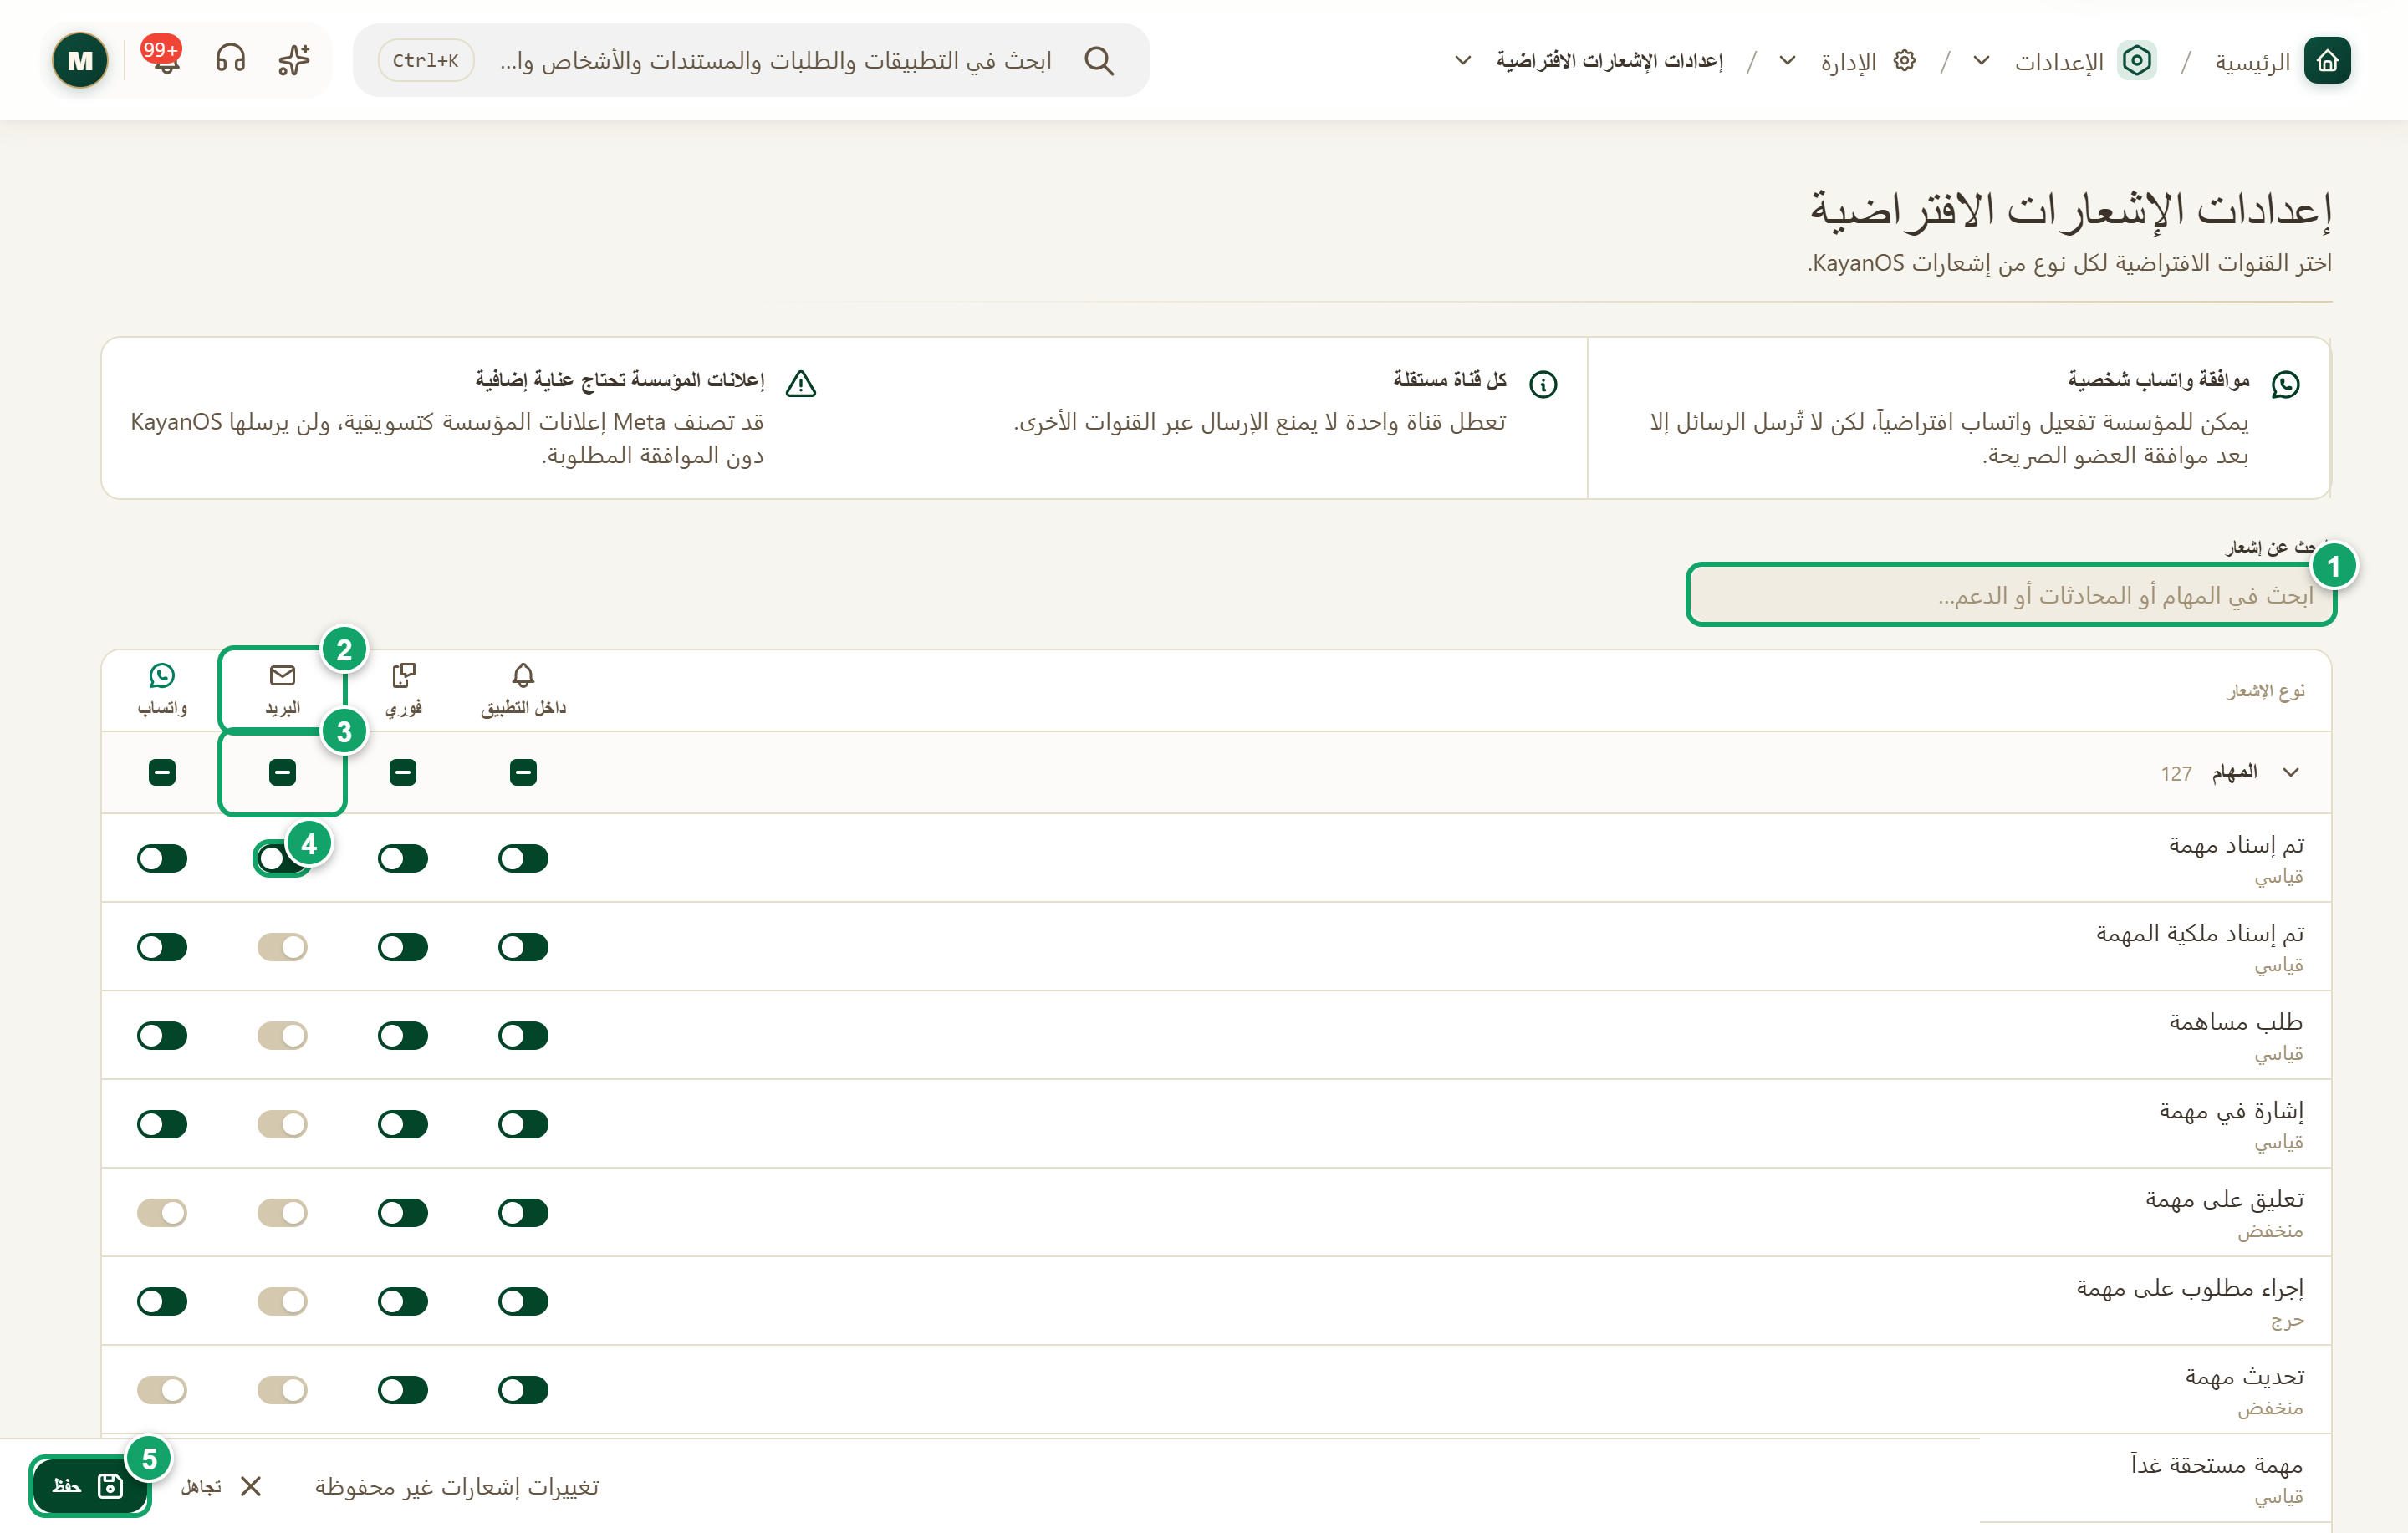
\includegraphics[width=0.95\linewidth,height=0.72\textheight,keepaspectratio]{figures/screens/ch08-notifications-ar.png}
\caption{جدول الإشعارات مع تغيير واحد لم يُحفظ}
\label{fig:settings-notifications-screen}
\shotnote{تعرض الصورة صفوف مجموعة «المهام» في مؤسسة الاختبار، وقد غُيّر مفتاح واحد لإظهار شريط الحفظ ثم أُلغي التغيير. فالصفوف أنواع الإشعارات، والأعمدة قنوات إرسالها، ولا يسري شيء قبل الحفظ. ① «البحث عن إشعار»: يبحث حالياً في أسماء إنجليزية داخلية، فلا يجد الكلمات العربية. ② عمود «البريد». ③ مربع المجموعة: يطبق القيمة على القناة في كل صفوف المجموعة، وتدل الشرطة داخله على قيم مختلفة. ④ مفتاح القناة لنوع إشعار واحد. ⑤ «حفظ»: يظهر مع «تجاهل» بعد أول تغيير.}
\end{figure}

\begin{table}[H]
\centering
\caption{ماذا تسجل في إعدادات الإشعارات الافتراضية؟}
\label{tab:settings-notifications-fields}
\begin{tabularx}{\linewidth}{R{4.2cm} Y}
\rcHeaderRow
\thh{العنصر} & \thh{ما الذي يعنيه؟}\\
«داخل التطبيق» & إشعار يظهر في قائمة الإشعارات داخل النظام.\\
«فوري» & تنبيه يصل إلى جهاز العضو.\\
«البريد» & رسالة إلى البريد الإلكتروني للعضو.\\
«واتساب» & رسالة واتساب، ولا تُرسل إلا بعد موافقة العضو الصريحة حتى لو فعّلتها المؤسسة.\\
المجموعات & تجمع الإشعارات بحسب مصدرها: «المهام» و«المحادثات» و«التقويم» و«البريد الإلكتروني» و«النظام» و«الدعم واتفاقية الخدمة» و«التوقيع» و«الحضور» و«المراسلات الرسمية».\\
درجة الإشعار & تظهر تحت اسمه: «منخفض» أو «قياسي» أو «عاجل» أو «حرج». وهي معلومة ثابتة لا تغيّرها من هنا.\\
الخلية الفارغة & قناة لا تتاح لهذا النوع من الإشعارات، فلا يظهر فيها مفتاح.\\
\end{tabularx}
\end{table}

\begin{figure}[H]
\centering
\begin{tikzpicture}[node distance=0.5cm]
\node[stepBox] (a) {\RL{اختيار العضو في حسابه، إن وُجد}};
\node[stepBox,below=of a] (b) {\RL{إعداد المؤسسة في هذه الصفحة، إن وُجد}};
\node[stepBox,below=of b] (c) {\RL{القيمة الأصلية في النظام}};
\draw[flowsTo] (a) -- (b);
\draw[flowsTo] (b) -- (c);
\end{tikzpicture}
\rclegend
\caption{أي قيمة تسري على العضو؟}
\label{fig:settings-notifications-order}
\shotnote{يبدأ النظام من اختيار العضو، فإذا لم يجده انتقل إلى إعداد المؤسسة، ثم إلى القيمة الأصلية. لذلك لا يغيّر حفظ هذه الصفحة ما اختاره العضو بنفسه. فإذا لم يصله إشعار فعّلته المؤسسة، فراجع اختياراته أولاً.}
\end{figure}

\begin{enumerate}
\item من «الإعدادات» افتح «إعدادات الإشعارات الافتراضية»، واقرأ الملاحظات الثلاث في أعلى الصفحة.
\item انتقل إلى المجموعة التي تريدها؛ فهي الطريق الأضمن إلى الإشعار، لأن حقل البحث لا يجد الكلمات العربية حالياً.
\item غيّر مفتاح القناة لنوع واحد، أو استخدم مربع المجموعة لتغيير الصفوف كلها.
\item اضغط «حفظ»، أو «تجاهل» لإلغاء التغييرات.
\end{enumerate}

\textbf{تحقق:} يختفي شريط «تغييرات إشعارات غير محفوظة» بعد الحفظ، وتبقى المفاتيح على قيمها الجديدة عند إعادة فتح الصفحة. وإذا ظهرت رسالة «تم تغيير الإعدادات من مكان آخر»، فقد حفظ شخص آخر قبلك؛ فاضغط «إعادة التحميل» وراجع القيم.

\clearpage
\section{مهام التصدير}
\label{sec:settings-feature-export-jobs}

تنشئ هذه الصفحة نسخة من بيانات المؤسسة في ملف \en{ZIP} يضم ملف \en{Excel} لكل نوع سجل، وتسمي الصفحة أنواع السجلات «الكيانات». وتفيدك عندما تحتاج إلى نسخة للأرشفة أو المراجعة أو التحليل خارج النظام. ولا يفتحها إلا مالك المؤسسة، لأن الملفات تحمل بيانات المؤسسة؛ فاحفظها في مكان آمن بعد تنزيلها.

\begin{rcnote}[مثال: شركة الأفق]
مسؤول النظام هو مالك المؤسسة في الأفق. يضغط «تصدير جديد» عند ①، ويختار سجلات الربع الأخير، ثم يعود حين تصبح الحالة «مكتملة» عند ③ وينزّل الملف عند ⑤ قبل انتهاء صلاحيته.
\end{rcnote}

\begin{figure}[H]
\centering
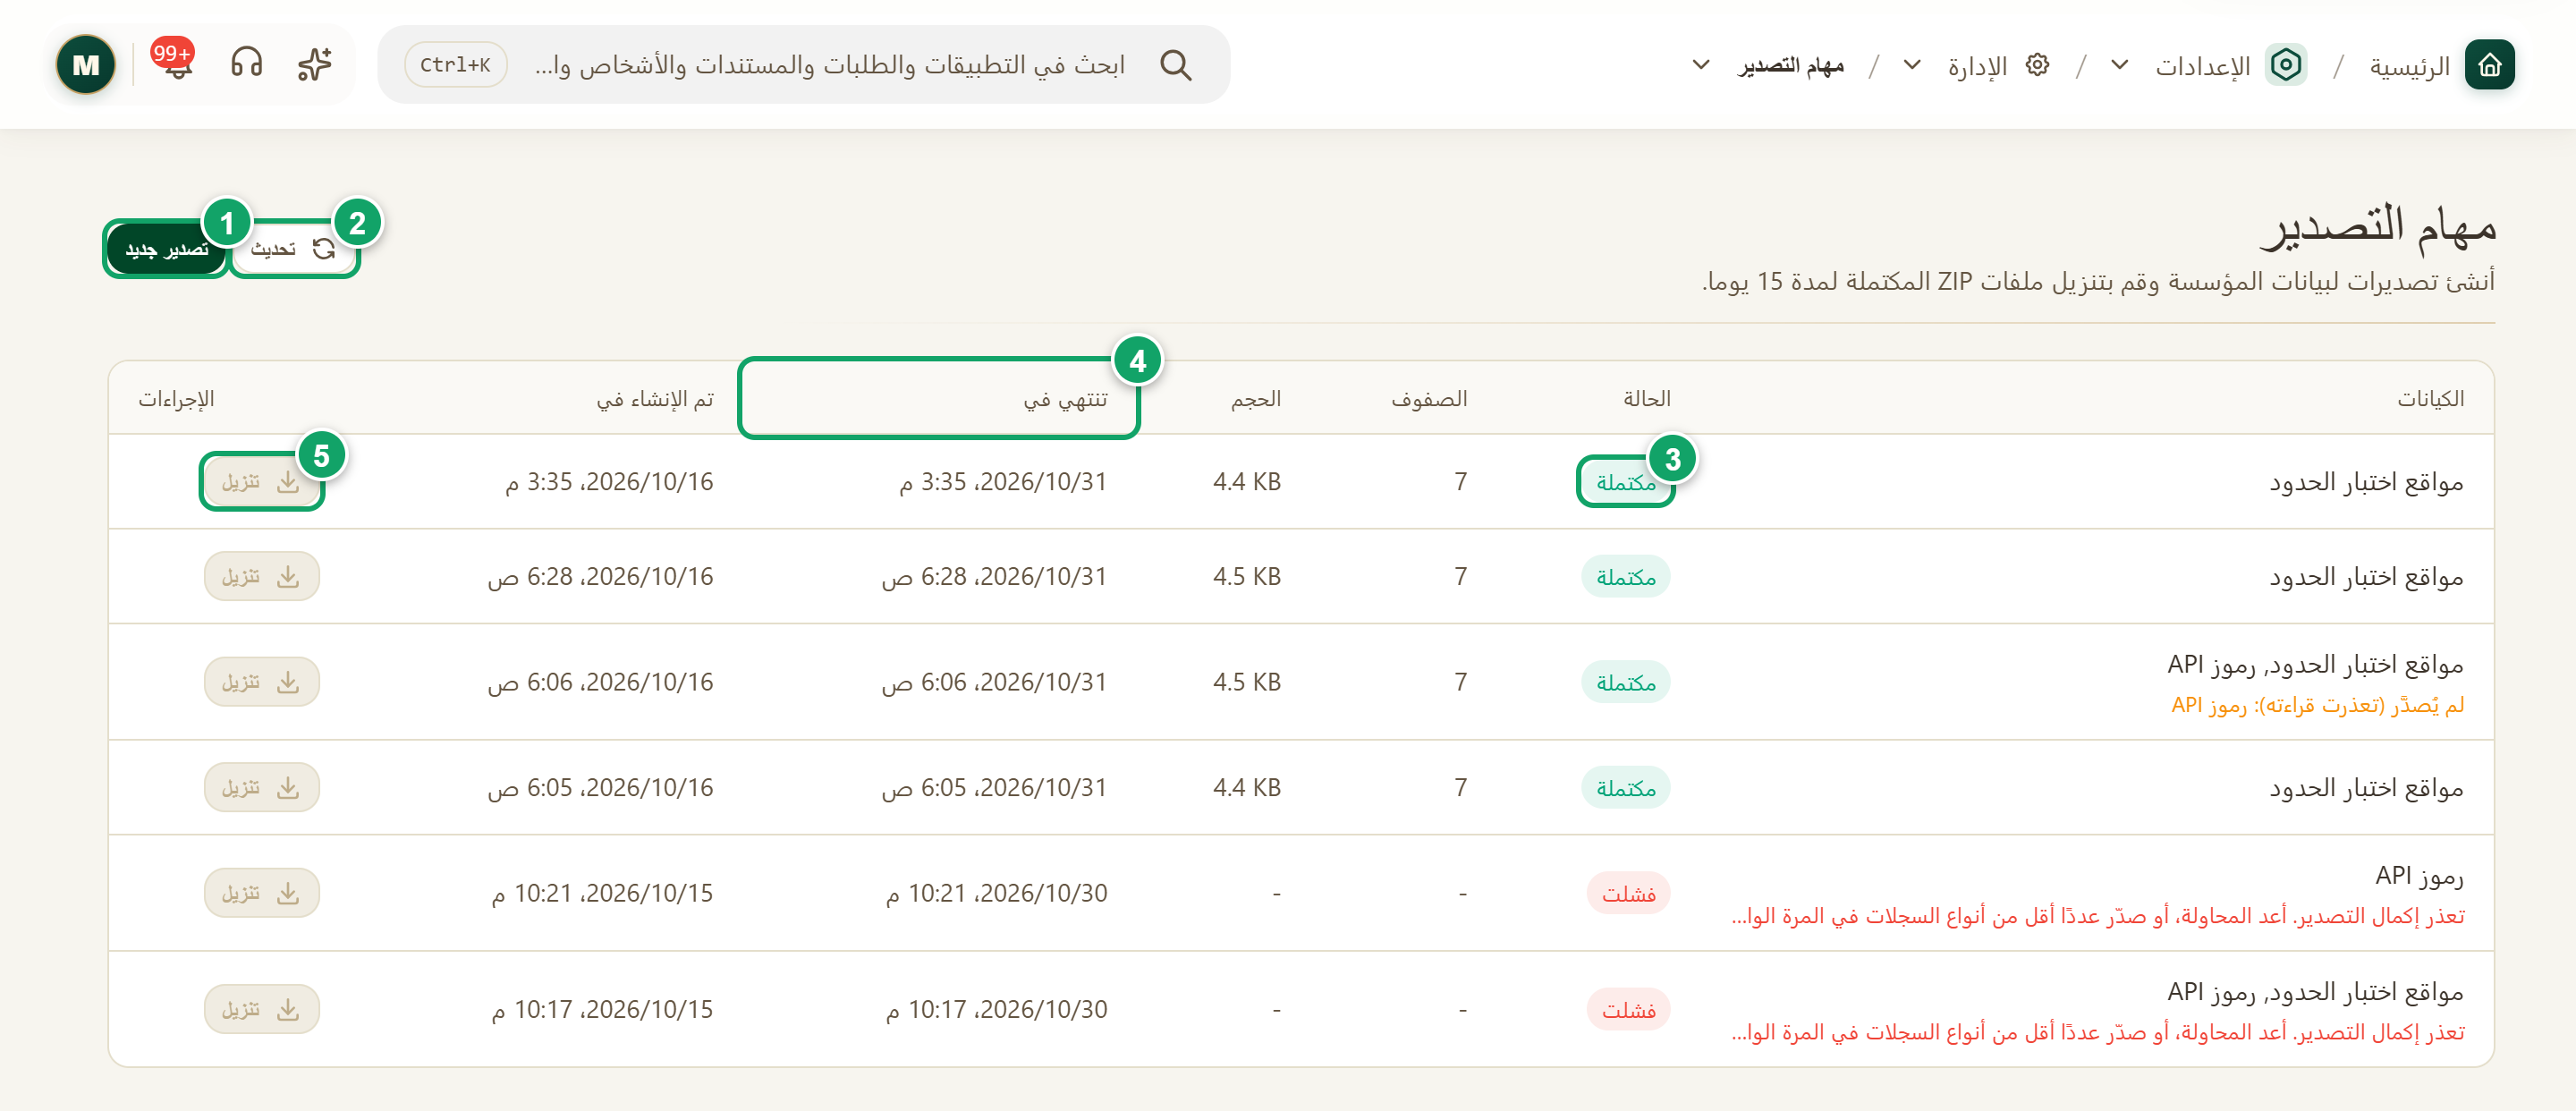
\includegraphics[width=0.95\linewidth,height=0.72\textheight,keepaspectratio]{figures/screens/ch08-export-jobs-ar.png}
\caption{قائمة مهام التصدير}
\label{fig:settings-export-jobs-screen}
\shotnote{تعرض الصورة مهام اختبار سابقة انقضت صلاحيتها، لذلك ظهرت أزرار «تنزيل» كلها معطلة. فالقائمة سجل لكل تصدير طلبته المؤسسة، وتبين حالته وحجمه والتاريخ الذي يتوقف فيه تنزيله. ① «تصدير جديد». ② «تحديث»: يعيد قراءة القائمة، وتتحدث وحدها كل عشر ثوانٍ أثناء العمل. ③ الحالة: «قيد الانتظار» ثم «قيد المعالجة» ثم «مكتملة» أو «فشلت». ④ «تنتهي في»: آخر موعد للتنزيل، بعد 15 يوماً من الإنشاء. ⑤ «تنزيل».}
\end{figure}

\begin{figure}[H]
\centering
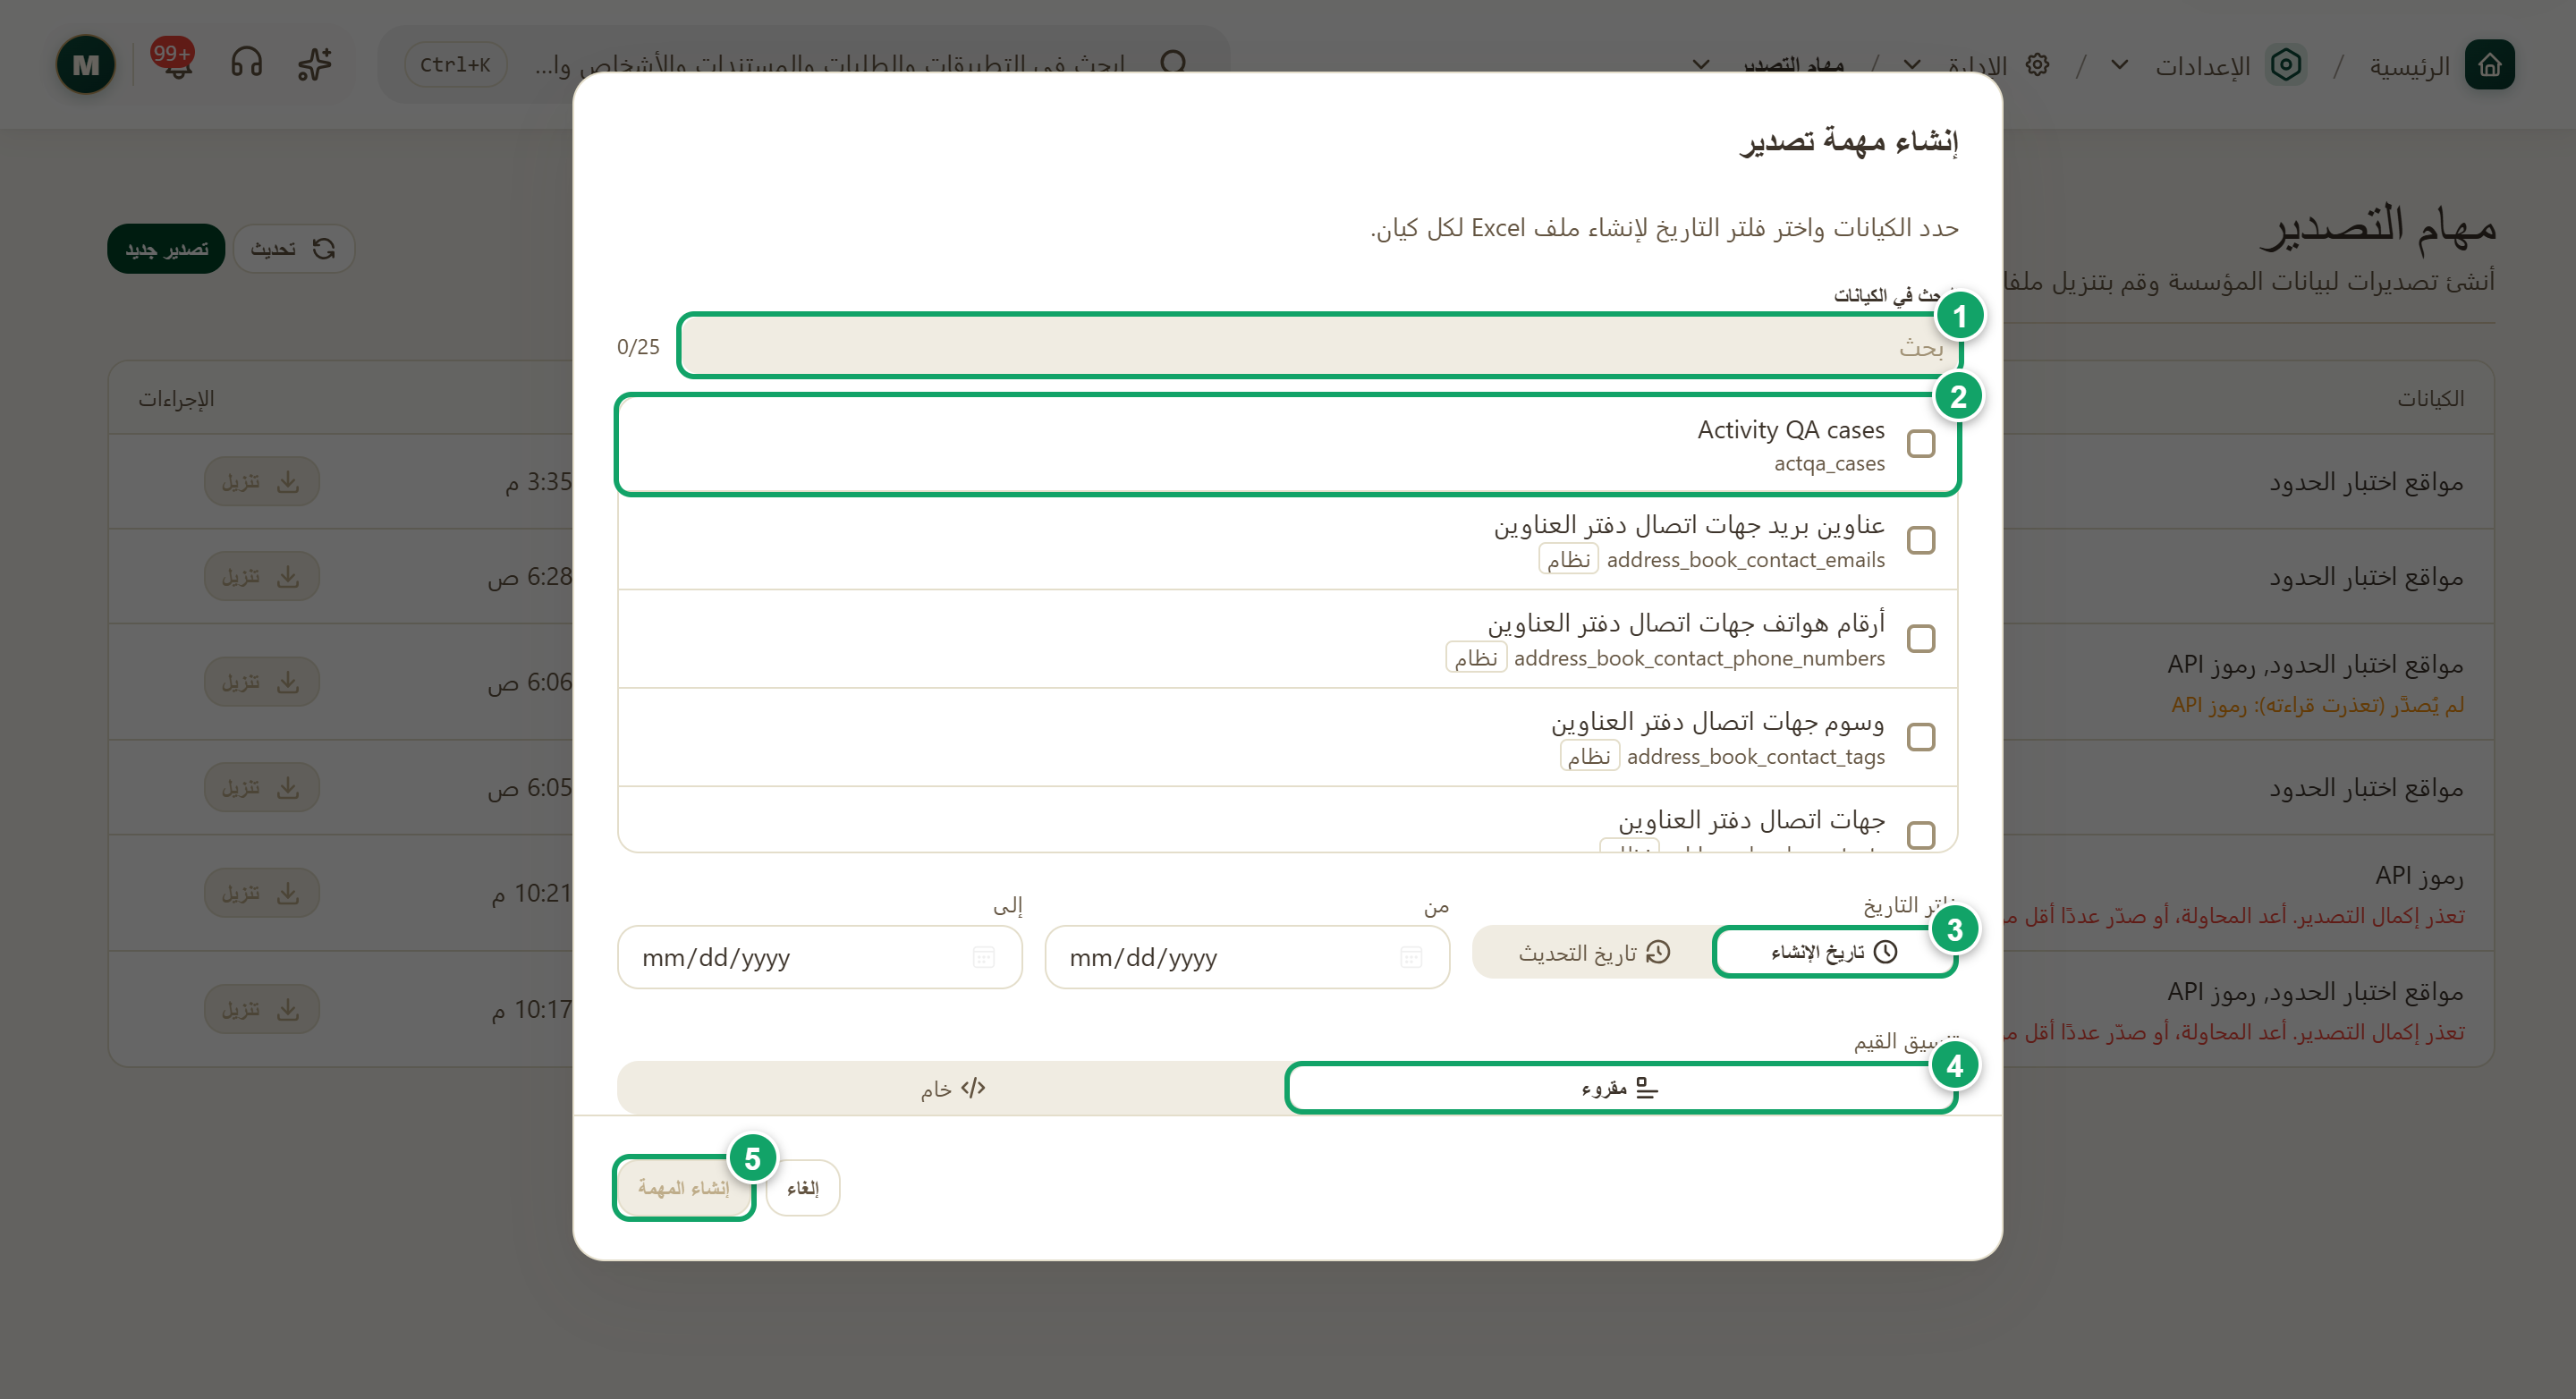
\includegraphics[width=0.95\linewidth,height=0.72\textheight,keepaspectratio]{figures/screens/ch08-export-jobs-create-ar.png}
\caption{نافذة إنشاء مهمة تصدير}
\label{fig:settings-export-jobs-create-screen}
\shotnote{تعرض الصورة النافذة قبل اختيار أي نوع، ولذلك يبقى زر الإنشاء معطلاً، والأسماء الظاهرة هي أسماء مؤسسة الاختبار. وتحدد اختياراتك هنا ما يدخل في الملف وكيف تظهر قيمه. وقد أُغلقت النافذة دون إنشاء مهمة. ① «البحث في الكيانات»، وبجانبه عداد المحددات من 25. ② نوع سجل يُحدَّد بالضغط عليه، وقد يحمل وسم «نظام» أو «أصلي». ③ «فلتر التاريخ». ④ «تنسيق القيم». ⑤ «إنشاء المهمة».}
\end{figure}

\begin{table}[H]
\centering
\caption{ماذا تسجل في مهمة التصدير؟}
\label{tab:settings-export-jobs-fields}
\begin{tabularx}{\linewidth}{R{4.2cm} Y}
\rcHeaderRow
\thh{الحقل} & \thh{ما الذي تسجله فيه؟}\\
الكيانات & أنواع السجلات المطلوبة، حتى 25 نوعاً في المهمة الواحدة.\\
«فلتر التاريخ» & هل تُقاس الفترة على «تاريخ الإنشاء» أم «تاريخ التحديث» في السجل.\\
«من» و«إلى» & حدود الفترة، وهما اختياريان. ويجب ألا يأتي تاريخ البداية بعد تاريخ النهاية.\\
«تنسيق القيم» & «مقروء» يعرض القيم كما يفهمها الموظف، و«خام» يعرضها كما هي مخزنة في النظام.\\
\end{tabularx}
\end{table}

\begin{enumerate}
\item من «الإعدادات» افتح «مهام التصدير»، ثم اضغط «تصدير جديد».
\item ابحث عن أنواع السجلات وحدّدها، ثم اختر «فلتر التاريخ» والفترة إذا أردت جزءاً من البيانات.
\item اختر «مقروء» للقراءة المباشرة، أو «خام» إذا كان الملف سيُنقل إلى نظام آخر.
\item اضغط «إنشاء المهمة»، وانتظر حتى تصبح الحالة «مكتملة»، ثم اضغط «تنزيل».
\end{enumerate}

\textbf{تحقق:} تظهر المهمة في القائمة، ثم يتفعل «تنزيل» عند اكتمالها. ولا تعمل في المؤسسة أكثر من مهمتين معاً. وإذا ظهر تحت الاسم «لم يُصدَّر (عدد السجلات كبير، اختر فترة زمنية أقصر)»، فقد تجاوز النوع 100 ألف سجل، فأعد تصديره بفترة أقصر. وإذا «فشلت» المهمة، فأعد المحاولة بعدد أقل من الأنواع.

\clearpage
\section{التقارير}
\label{sec:settings-feature-reports}

تجمع هذه الصفحة القيم التي يبدأ بها كل تقرير: الفترات، وعرض العملة، وطريقة إرسال التقارير وحفظها، ومفاتيح لوحة المفاتيح. وبذلك لا يكرر مصمم التقرير هذه القرارات، ولا يرسل تقريراً عبر قناة لا تسمح بها المؤسسة. تحمل الصفحة وسم «تجريبي»، وتظهر لمالك المؤسسة ولمن يحمل دور المسؤول، وهم وحدهم يغيّرون قيمها.

\begin{rcnote}[مثال: شركة الأفق]
يُبقي مسؤول النظام «رابط آمن» عند ③ والبريد الإلكتروني مسموحين، ويترك واتساب متوقفاً، ثم يضغط «حفظ» عند ⑤. وعندما يُعدّ عمر حداد تقريره الشهري، لا تتاح له قناة واتساب.
\end{rcnote}

\begin{figure}[H]
\centering
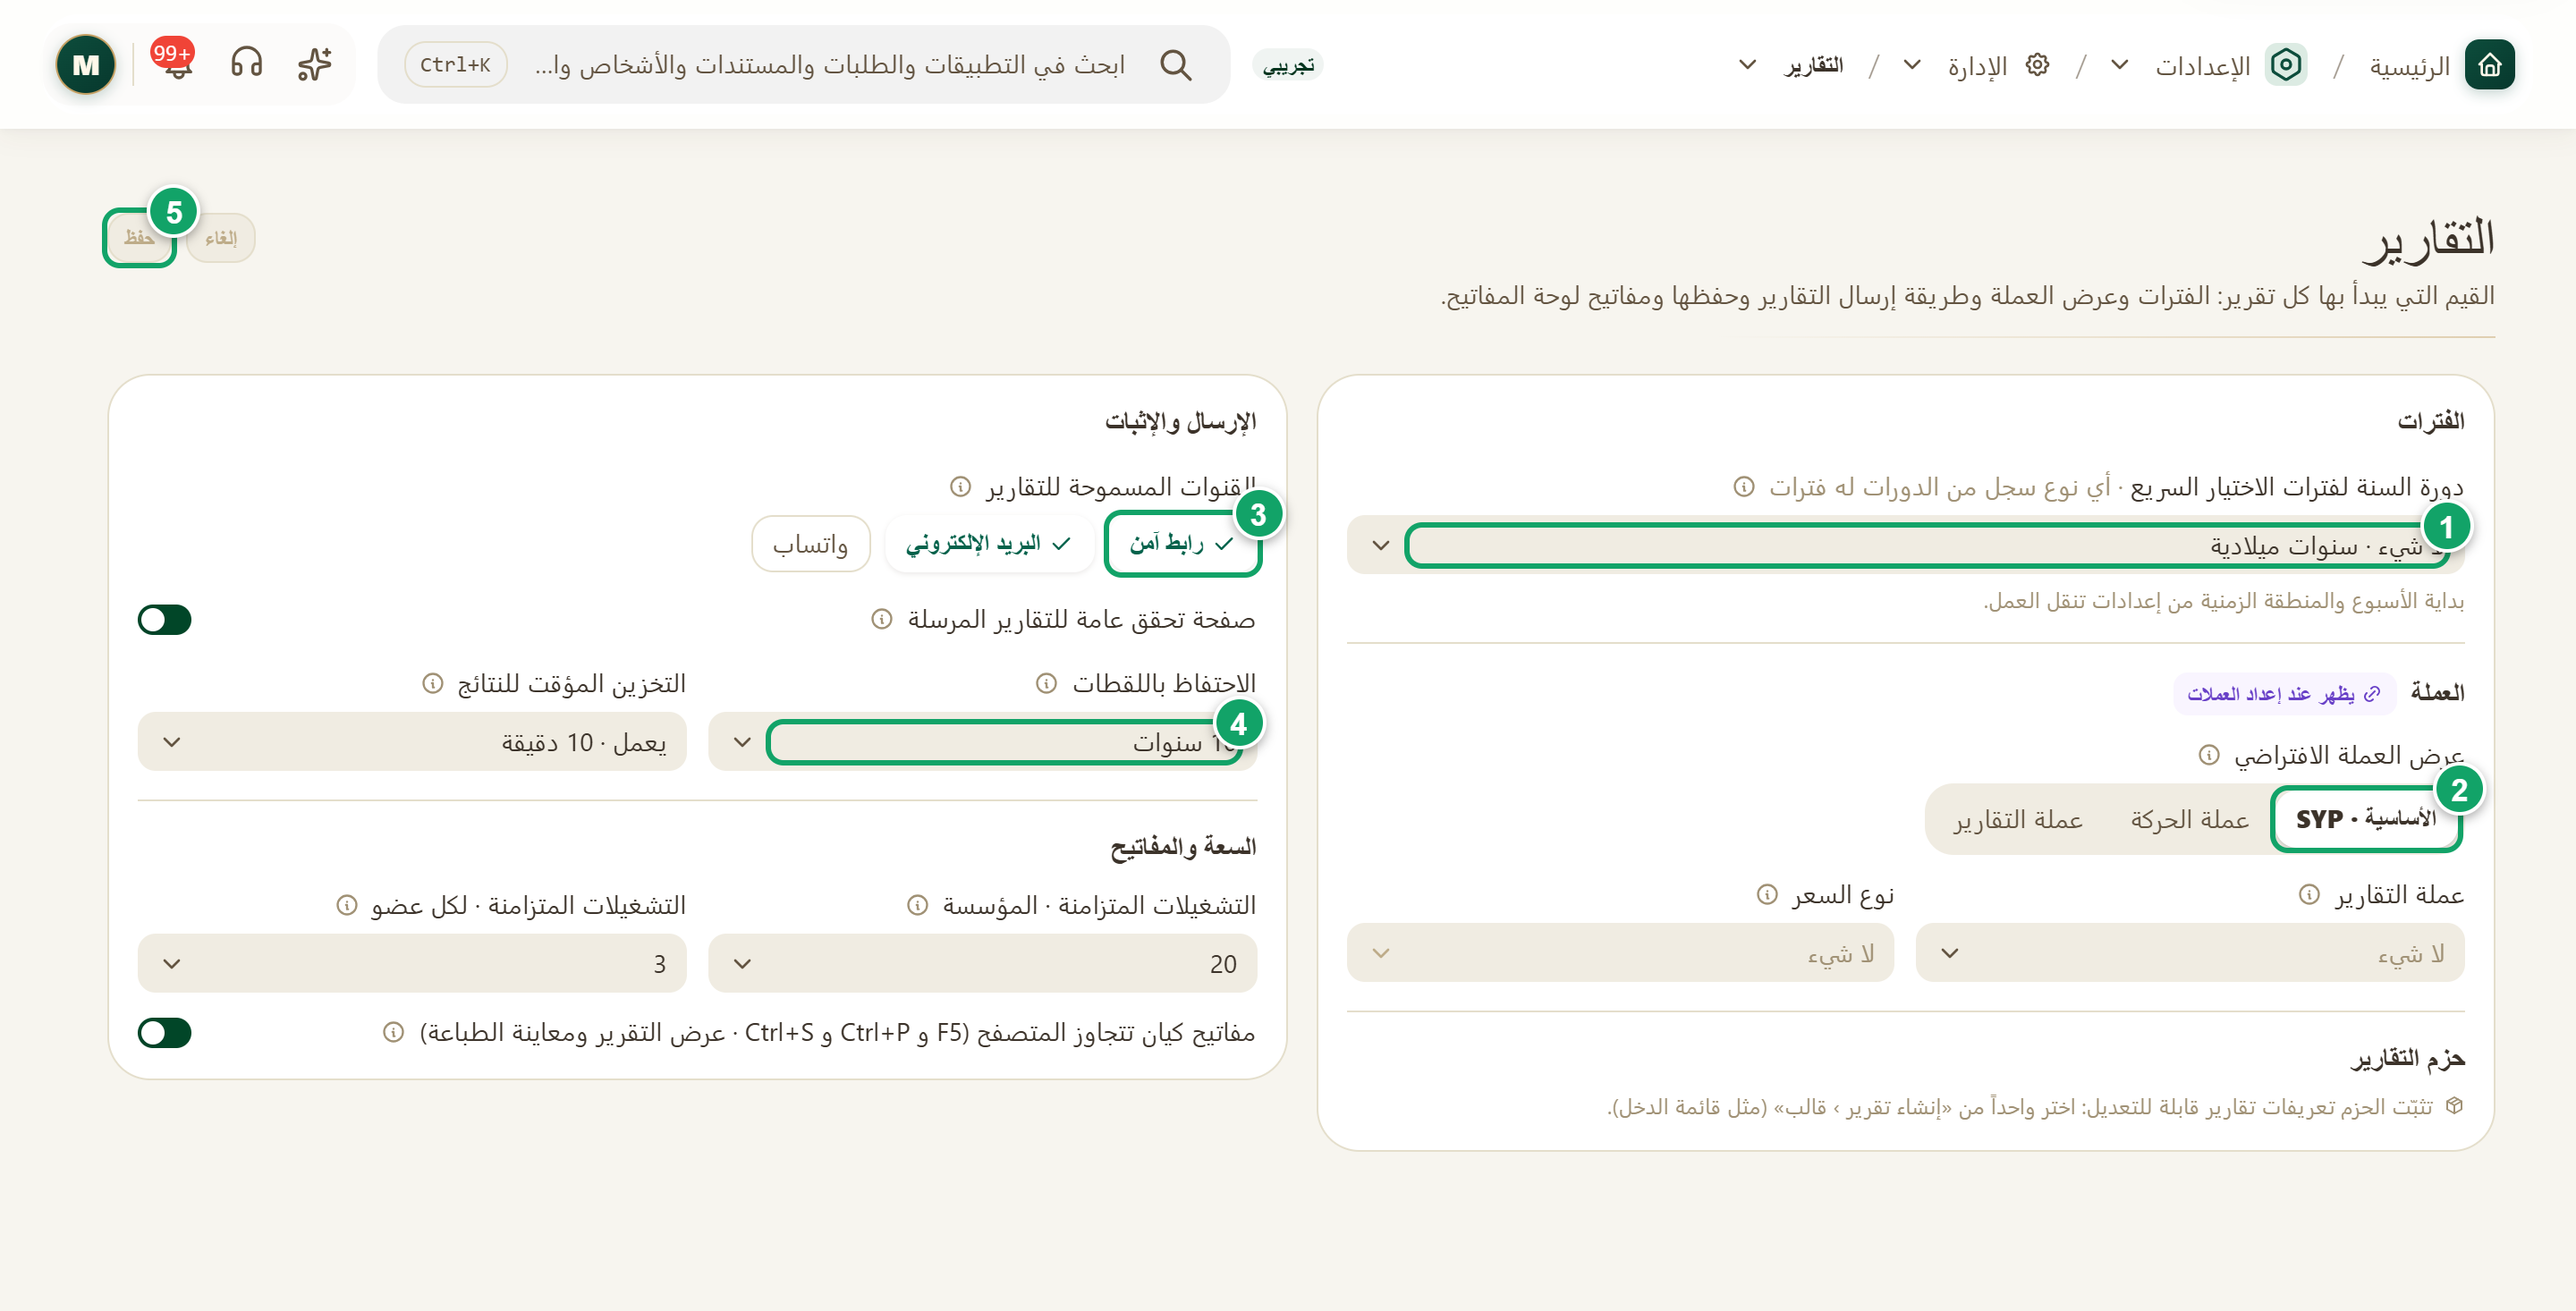
\includegraphics[width=0.95\linewidth,height=0.72\textheight,keepaspectratio]{figures/screens/ch08-reports-ar.png}
\caption{إعدادات التقارير}
\label{fig:settings-reports-screen}
\shotnote{تعرض الصورة قيم مؤسسة الاختبار، وعملتها الأساسية \en{SYP}. تنطبق هذه القيم على التقارير كلها، وأهمها القنوات لأن إيقاف قناة يمنعها في جميع التقارير. أما بداية الأسبوع والمنطقة الزمنية للفترات فتأتيان من «إعدادات تنقل العمل» لا من هذه الصفحة. ① «دورة السنة لفترات الاختيار السريع»: القيمة الحالية سنوات ميلادية. ② «عرض العملة الافتراضي». ③ «القنوات المسموحة للتقارير»: اضغط القناة لتشغيلها أو إيقافها. ④ «الاحتفاظ باللقطات». ⑤ «حفظ»: يتفعل مع «إلغاء» بعد أول تغيير.}
\end{figure}

\begin{table}[H]
\centering
\caption{ماذا تسجل في إعدادات التقارير؟}
\label{tab:settings-reports-fields}
\begin{tabularx}{\linewidth}{R{4.2cm} Y}
\rcHeaderRow
\thh{الحقل} & \thh{ما الذي تسجله فيه؟}\\
«دورة السنة لفترات الاختيار السريع» & نوع سجل الدورات الذي تحدد فتراته «هذه السنة» و«من أول السنة» و«هذه الفترة». وبدونه تُستخدم السنوات الميلادية.\\
«عرض العملة الافتراضي» & «الأساسية» أو «عملة الحركة»، أي عملة كل سطر، أو «عملة التقارير» المحوّلة.\\
«عملة التقارير» و«نوع السعر» & العملة التي تُحوَّل إليها المبالغ والسعر المستخدم. وإذا غاب السعر توقف التقرير برسالة واضحة.\\
«حزم التقارير» & ملاحظة لا تحتاج إلى إدخال: تُثبَّت الحزم من «إنشاء تقرير › قالب».\\
«القنوات المسموحة للتقارير» & «رابط آمن» و«البريد الإلكتروني» و«واتساب».\\
«صفحة تحقق عامة للتقارير المرسلة» & تحمل النسخة المرسلة رابطاً ورمز \en{QR} لصفحة تُظهر أن أرقامها صادرة عنكم ولم تتغير.\\
«الاحتفاظ باللقطات» & مدة حفظ النسخ الثابتة من التقارير، من سنة إلى 20 سنة.\\
«التخزين المؤقت للنتائج» & يحفظ النتيجة حتى ساعة ليصبح فتحها مجدداً أسرع، أو اختر «متوقف». وأي ترحيل جديد يلغي النتيجة المحفوظة.\\
«التشغيلات المتزامنة» & عدد التقارير التي تعمل معاً: من 5 إلى 50 للمؤسسة، ومن 1 إلى 5 لكل عضو، وينتظر الباقي دوره.\\
«مفاتيح كيان تتجاوز المتصفح» & في التقرير ومعاينة الطباعة يحدّث \en{F5} التقرير، ويطبعه \en{Ctrl+P}، ويحفظ \en{Ctrl+S} خياراته بدل المتصفح.\\
\end{tabularx}
\end{table}

\begin{enumerate}
\item من «الإعدادات» افتح «التقارير»، ثم راجع قسم «الفترات».
\item اختر عرض العملة. وإذا اخترت «عملة التقارير»، فحدّد العملة ونوع السعر.
\item حدّد القنوات المسموحة وصفحة التحقق ومدة الاحتفاظ والتخزين المؤقت.
\item راجع قسم «السعة والمفاتيح»، ثم اضغط «حفظ»، أو «إلغاء» للرجوع إلى القيم المحفوظة.
\end{enumerate}

\textbf{تحقق:} تظهر رسالة «حُفظت إعدادات التقارير.» ويتعطل الزران حتى التغيير التالي. وعند إرسال تقرير، لا تعمل القناة التي أوقفتها. وإذا فتح الصفحة عضو آخر عبر رابطها، تظهر له رسالة «يغيّر إعدادات التقارير المالكون والمسؤولون فقط.» وتكون الحقول معطلة.
